Chapter \ref{ch:approach} has formalized the problem and put forward a novel framework for finding useful words, consisting of two major functionalities:
Vocabulary list generation, and vocabulary list evaluation.
The list evaluation approach, described in Section \ref{sec:experimental-setup-with-ai}, utilizes the performance of an AI model in an NLP task on a context-specific corpus as a proxy metric for language ability, in order to estimate how efficiently the vocabulary list may help a human language learner in acquiring language competency.
The list generation approach, proposed in Section \ref{sec:list-generation}, additionally uses Explainable AI as a tool for analyzing the interaction of the AI model with the corpus to compile vocabulary lists that approach maximal efficiency.

In this chapter, we describe our implementation, especially of the list generation approach.
This is because the list evaluation method is used in Chapter \ref{ch:evaluation} as one among several metrics for evaluating the efficiency of vocabulary lists generated by the implementation described in this chapter.
However, our implementation of the evaluation approach uses the same AI models and Corpora as the list generation approach.

We first discuss the implementation of the list generation approach from an abstract perspective in Section \ref{sec:data-pipeline}, describing how we generate lists of vocabulary, without elaborating on the interdependencies that arise between concrete NLP tasks, corpora, and XAI methods.
The choice of those three components in the system is then argued in the following sections, each of which features a subsection where we discuss desiderata of the specific component on the basis of our aim as stated in Section \ref{sec:formal-problem-statement}, followed by the selection of concrete components.
Finally, we return to the holistic perspective in Section \ref{sec:implementation-final}, where we present the complete implementation with all individual components integrated.

\section{Data Pipeline} \label{sec:data-pipeline}

This section gives a top-level overview of our implementation for the list generation approach described in Chapter \ref{ch:evaluation}.
As mentioned before, the main components of this approach are:

\begin{itemize}
	\item An AI model, used as a test subject.
	\item An NLP task, the score in which is used as a proxy metric for the language ability of the test subject.
	\item A context-specific corpus, to model a language context.
	\item An XAI method, which analyzes the interaction of the AI model with the corpus to determine word utilities.
\end{itemize}

In addition, we must perform some pre-processing in the form of tokenization on the input texts for model-agnostic methods, which determines the words to be analyzed.
Thus, the implementation of the approach mainly consists of deciding which AI model, XAI method, etc., is used, as well as determining how exactly these components interact with each other.
In addition, we perform pre-processing on the lines from the corpora, the exact form of which is dependent on the XAI method used.
The interaction of these components can be seen in pseudocode in Algorithm \ref{alg:efficient-list-generation}.

\begin{algorithm}
\caption{Efficient List Generation.}
\label{alg:efficient-list-generation}
\begin{algorithmic}[1]
\Require corpus, model, xai\_method
\State Initialize $line\_word\_utilities$ with empty list

\For{each $line$ in $corpus$}
    \State $word\_utilities\_for\_this\_line \gets$ xai\_method$(model, line)$
    \State Append $word\_utilities\_for\_this\_line$ to $line\_word\_utilities$
\EndFor

\State $corpus\_word\_utilities \gets$ aggregate($line\_word\_utilities$)
% \State $corpus\_word\_utilities\_scores$ $\gets$\newline
% aggregate\_word\_utilities($line\_word\_utilities\_scores$)

\State $voc\_list \gets$ words ordered by $corpus\_word\_utilities$

\State \Return $voc\_list$
\end{algorithmic}
\end{algorithm}


The XAI method outputs the importance attributions in the form of one number for each unique word in each input line.
The results are aggregated by taking the sum across all lines in the corpus, resulting in a list of word-utility pairs, which reflect the estimated utility of the word with respect to the entire corpus.
To make a vocabulary list from these words, we simply order the words by their estimated corpus utility in descending order.

With this basic structure established, the following sections address the selection of individual components.
Due to the interdependencies between certain components, not all are presented in separate sections.
The NLP task performed depends on the AI model that we use, as most AI models are trained on only one task.
Therefore, the choice of AI model is discussed together with the NLP task in a single section.

\section{Pre-Processing}
This section describes our pre-processing performed on the input lines to the AI models, namely tokenization to split the lines into words from which to build the vocabulary lists, and named entity recognition to minimize the occurrence of personal and place names in the lists.
As this is a rather minor part of the implementation, the descriptions are brief.

\subsection{Tokenization}
For tokenizing the input lines, we use the \texttt{bert-base-uncased} tokenizer \footnote{\url{https://huggingface.co/google-bert/bert-base-uncased}}, which is a case-insensitive tokenizer for English.
One disadvantage of this tokenizer is that it splits English contractions such as \texttt{don't} and \texttt{I've} into the sub-word tokens \texttt{["don", "'", "t"]} and \texttt{["i", "'", "ve"]}, respectively, leaving no indication that these sub-word tokens once formed a complete word.
For this reason, our generated vocabulary lists contain the constituents of these contractions, instead of the complete words.
While we could merge these contractions manually, we wanted to perform the experiments with minimal manual intervention, in order to form a conception of the capabilities of our implementation when applied to languages without expert intervention.

\subsection{Named Entity Recognition}
For named entity recognition, we used the pre-trained English model \texttt{en\_core\_web\_sm} \footnote{\url{https://spacy.io/models/en}} from the Python package \texttt{spacy}.
\texttt{spacy} also contains the multilingual model \texttt{xx\_ent\_wiki\_sm} \footnote{\url{https://spacy.io/models/xx\#xx_ent_wiki_sm}}, which supports 9 languages and which we would have used if we had evaluated our pipeline on other languages than English.
This model is context-dependent, meaning it relies on surrounding text to recognize named entities with full accuracy.
For this reason, we do not filter the lists after they have been compiled; rather, we use the model on the input lines to the AI models.
The model outputs the character ranges of named entities it recognizes, which we use to filter out the tokens in the ranges in question.

\section{NLP Tasks and AI Models}
Our approaches for list efficiency evaluation and for efficient list generation use an AI model with an NLP task to simulate a test subject performing a language exam.
Because of this, the AI model and NLP task are a crucial component of these approaches, and their appropriate selection is essential to the implementation.
The NLP tasks we choose also influence what corpora we can use for their execution:
The task of next sentence prediction requires contiguous texts as input data, necessitating input corpora containing whole documents, not just individual sentences.

This section first puts forward criteria for selecting NLP tasks in Section \ref{sec:nlp-tasks-desiderata} for word utility evaluation.
% After this, we use these criteria to select a few NLP tasks as appropriate in Section \ref{sec:nlp-tasks-selection}.
We then discuss potential candidate NLP tasks, and discuss how appropriate they are for our approach.
Finally, we select two tasks which, in the estimation of the author of this work, are suitable for our word utility evaluation approach, namely \textit{next sentence prediction} and \textit{sentence embedding}.

\subsection{Desiderata} \label{sec:nlp-tasks-desiderata}

This section puts forward four criteria for selecting NLP tasks for word utility evaluation, arising from our underlying goal of using the task as a proxy for real language interaction of a human being:
Our selection is a matter of how many languages AI models and corpora usable by the task are available, how reflective of real language ability we estimate the task to be, and how easy is its evaluation.
These criteria are used in Section \ref{sec:candiate-tasks-survey} to select concrete tasks for our implementation.

\subsubsection{Model Availability in Many Languages}
The goal of this work is to find approaches to find useful words for the purpose of language learning.
Much research in Natural Language Processing is dedicated to improving NLP performance in English and other high-resource languages such as English, French or Mandarin Chinese \cite{joshiStateFateLinguistic2021}.
This has the consequence that many AI models and other NLP methods achieve high levels of performance only in these languages, and many AI models are only available in English or only a small number of languages \cite{joshiStateFateLinguistic2021}.
However, there are over 7,000 languages in the world \footnote{According to \textit{Ethnologue} (\url{https://www.ethnologue.com/}, last accessed on April 22, 2025)}, and for many of these there exist corpora, or online digital texts which can be used as inputs for our word utility evaluation approach, such as Wikipedia articles, \textit{Open Parallel Corpora}  (OPUS) \footnote{\url{https://opus.nlpl.eu/}}, or \textit{Wortschatz Leipzig} \footnote{\url{https://wortschatz.uni-leipzig.de/}}.
In order to make an implementation with the potential to exploit the linguistic diversity in these resources to the fullest extent, we only consider NLP tasks for which pre-trained models exist which can process a high number of languages.

\subsubsection{Corpus Availability in Many Languages}
The second point of consideration for task selection is \textbf{how much data is available for performing the task}.
Ideally, we would like tasks for which suitable corpora are freely available or can be trivially generated from available corpora.
This is because, with a larger amount of usable data, we not only improve the accuracy of our approach, but also increase the diversity of input data.
Because context-specific language learning is a central motivation of this work, diverse training data is desirable, as it provides a broader range of linguistic contexts to model and from which to identify useful words.

\subsubsection{Generality of Skill Required}
Another important point to consider when selecting an NLP task is \textbf{how general the linguistic skills} are that the task requires:
We use the performance in the NLP task as a proxy metric for the test subject's language ability.
As such, we must ensure that task reflects a general level of semantic understanding, not only a narrow mechanistic skill that can be accomplished by using only a small part of the input.
For this reason, we do not consider tasks such as part-of-speech tagging and text classification appropriate, as they do not reflect skills of language speakers used in everyday life.

\subsubsection{Ease of Evaluation} \label{sec:ease-of-evaluation}
To ensure we can measure task performance, we must also choose a task whose results can be easily compared with each other:
Some tasks are difficult to evaluate objectively, or the evaluation takes an inordinate amount of computation (see Section \ref{sec:text-summarization} on text summarization).
It follows that if we have the freedom to choose NLP tasks whose results can be automatically evaluated with good accuracy, we should choose them.


\subsubsection{Summary of Desiderata}
To summarize our desiderata for NLP tasks:
Our implementation seeks to use NLP tasks for which AI models and Corpora exist in a large number of languages, to make our approach for finding useful vocabulary usable in the greatest number of languages.
We prefer tasks that demonstrate general language understanding over tasks that only require a narrow skill set to perform, because these are expected to align more with human linguistic skills.
Finally, the task must be easily scorable, since analyzing the changes in the task score is how we gauge the utility of words.
The next section introduces several candidate tasks, primarily by surveying which tasks are commonly used as pre-training tasks for state-of-the-art language models, as these must fulfill similar requirements to those stated in this section.

\subsection{Survey of Candidate NLP Tasks} \label{sec:candiate-tasks-survey}
This section introduces several NLP tasks we use in our implementation, as well as some tasks which were not selected.
We first describe the process of how candidate tasks were found, and then go into detail for each candidate as to why it was or was not selected in the following subsections.

Candidates were first compiled by surveying common pre-training tasks which are used in state-of-the-art NLP models:
This is because the purpose of a pre-training task is to endow the AI model with a general understanding of the language, before using transfer learning to specialize it for a more specific downstream task \cite{jurafskySpeechLanguageProcessing2025a}.
Such tasks necessarily require general language understanding of a kind, since training the model with them is supposed to provide a solid basis for a wide variety of NLP tasks.
Another benefit of using pre-training tasks is that their training is unsupervised, meaning there is no need to manually label data.
Their widespread use in \NLP\ also means that pre-trained models are widely and freely available.
From this consideration, we consider language modeling and next sentence prediction as candidates, but reject language modeling for the reasons described below.
In addition to these common pre-training tasks also consider text summarization and sentence embedding.
However, because text summarization is difficult to evaluate, we reject this task as well.

\subsubsection{Language Modeling}
There generally exist two subtypes of language modeling, namely Causal Language Modeling and Masked Language Modeling \cite{jurafskySpeechLanguageProcessing2025a}.
Causal language modeling describes the task of predicting the next token in a text, given the sequence of previous tokens, and it constitutes the basis of many recent developments in Large Language Models \cite{brownLanguageModelsAre2020} \cite{openai2024gpt4technicalreport}.
Masked language modeling involves filling in missing tokens in a sentence, and is one of the training tasks for the popular BERT models \cite{kentonBertPretrainingDeep2019}, along with next sentence prediction.

While its training data can be trivially generated from corpora and does not pose great challenges in evaluation, we did not consider either type of language modeling an appropriate NLP task for the purpose of finding useful vocabulary.
This is because generating the task's training data already involves removing tokens from the input, resulting in training data with word distributions which do not correspond to language found in real texts.
Another issue arises to the nature of model-agnostic, feature importance attribution XAI methods:
These methods perturb the input to determine which tokens in the input are the most relevant.
However, whether or not a token is appropriate as the next token in a document changes with even slight perturbations:
Consider the sentence:

\begin{quote}
	\textit{The sky is blue.}
\end{quote}

A language model, given the input datum \textit{The sky is}, may be able to predict that \textit{blue} is a probable next word to this sentence.
However, if we mask the --- relatively unimportant --- word  \textit{is} in the sentence to find out if the model's can predict the last word of the sentence even when \textit{is} is missing, we are left with the sentence:

\begin{quote}
	\textit{The sky}
\end{quote}

For this variation, \textit{blue} is no longer an appropriate next word to predict, as this would result in a grammatically incorrect sentence.
This would lead a feature importance attribution method to evaluate \textit{is} as a very important word in the sentence, because its absence leads to a loss of accuracy, despite it being rather unimportant to the overall meaning of the sentence.
These complications make it difficult to use feature importance attribution methods on language modeling, which is why we decide against the use of this task for our implementation.


\subsubsection{Next Sentence Prediction} \label{sec:nsp}
In next sentence prediction (NSP for short), the AI model takes as input two sentences and predicts a probability for the second sentence being the successor of the first sentence in their source text \cite{kentonBertPretrainingDeep2019}.
Input data for this task, including labels, is trivial to generate from document-level corpora, as it merely requires a corpus of contiguous sentences (sentences which follow each other similarly to those the model was trained on), which is easily obtained from Wikipedia articles and most other kinds of continuous text.
As the output of next sentence prediction is one number expressing the predicted probability of the input sentences following each other, its outputs are also easily evaluated using cross-entropy or, for comparing two outputs, the simple difference between the two probabilities.
While predicting whether two sentences are consecutive may not seem like a transferable skill, it is used as one of two pre-training tasks for BERT models \cite{kentonBertPretrainingDeep2019}, which suggests that using this task in pre-training imbues the model with transferable language skills.
For these reasons, we use the NSP task in our word evaluation approach.


\subsubsection{Text Summarization} \label{sec:text-summarization}
This task involves summarizing a given text, in other words, writing a shorter version of the input text while still conveying as much of the information from the original text as possible \cite{radevIntroductionSpecialIssue2002}.
Summarizing texts accurately would seem to require a high level of understanding of the text, and thus be good choice for testing whether ablating certain words from the text has detrimental effect on the model performance.
Unfortunately, this task is not appropriate for our purposes with respect to our last desideratum, because evaluating the quality of a summary or comparing two summaries is a very challenging task:
Evaluation involves a ground truth summary which is usually manually created, against which another summary is compared.
This already makes the use of this task problematic for low-resource languages (languages for which only few or only small NLP datasets exist), as text summarization datasets are scarce for these \cite{dahanStateFateSummarization2025}.
However, even assuming sufficient data, the comparison of two summaries is difficult:

A standard way of evaluating summaries are ROUGE scores \cite{allahyariTextSummarizationTechniques2017}:
These measure the overlap of n-grams (word sequences) between two texts.
However, it is questionable how well they capture the similarity between texts, because they do not recognize the semantic similarity of synonyms, and a different sentence structure will result in a low ROUGE score even if the actual meaning of the sentences may be very close.
For these reasons, we do not use text summarization in our implementation.

\subsubsection{Sentence Embedding} \label{sec:sentence-embedding}
Sentence embedding takes sentences as inputs and outputs vectors of numbers, which are typically used as inputs for a downstream task such gauging the similarity between two sentences, which can in turn be used to find similar sentences across languages for making training data for translations model \cite{artetxeMassivelyMultilingualSentence2019} \cite{reimersMakingMonolingualSentence2020}.
This approach can be performed on any corpus containing distinct sentences, meaning the corpus does not have to be document-level, and sentences need not be consecutive.

An important characteristic of this task is that it has no ground truth labels, and therefore, when using feature importance attribution XAI methods, we cannot measure differences in performance of the downstream task when the input is perturbed.
Instead, we embed an input sentence in its original form (the baseline embedding), then embed variations of the sentence with some of its words removed, and measure the cosine distance (a usual distance measure for sentence embeddings \cite{reimersMakingMonolingualSentence2020}) between the baseline embedding and the embedding of each variation.
A large distance between the baseline and the variant embedding where a word has been removed implies that the removed word is useful for understanding the sentence.
We believe these distances are a valid metric for determining how much a word contributes to the meaning of the sentence, as the embedded vector is a semantic representation of the input.
In our estimation, the ease of evaluation and of finding input data, as well as its generality make sentence embedding an ideal task for word utility evaluation, which is why we use it not only for the generation of vocabulary lists, but also for the evaluation of their efficiency.

\subsection{Choice of Model}
In the previous sections, we have presented two tasks which seem appropriate choices for our vocabulary list generation and evaluation approach, namely, next sentence prediction and sentence embedding.
This section discusses the choice of the AI model used for both of these tasks.
The models in our implementation are monolingual models, as these have shorter inference times than their multilingual counterparts, allowing us to process more data.
However, we use models from model families which, in principle, support many languages, allowing for easy inclusion of additional languages in our implementation.

\subsubsection{Next Sentence Prediction Model}
As our next sentence prediction model, we use a BERT model \cite{kentonBertPretrainingDeep2019}, as these models have been trained in many languages (over 104 for \texttt{bert-base-multilingual-cased}, the model with the most languages \footnote{\url{https://huggingface.co/google-bert/bert-base-multilingual-cased}}).
However, for our implementation, we employ the monolingual English model \texttt{bert-base-uncased} \footnote{\url{https://huggingface.co/google-bert/bert-base-uncased}} (not to be confused with the tokenizer of the same name) for its smaller size (110M parameters instead of 170M for \texttt{bert-base-multilingual-cased}) and shorter inference time.
As BERT models form a family, their model architecture is similar to each other, making the extension of our approach to more languages trivial, even when using transformer attention as model-specific XAI method for vocabulary list generation (see Section \ref{sec:transformer}).


\subsubsection{Sentence Embedding Model}
For the sentence embedding task, there are two model families that appear as promising candidates for our implementation:
\textit{LASER} \cite{artetxeMassivelyMultilingualSentence2019}, developed by Meta, and \textit{Sentence Transformers} a.k.a. \textit{sBert} \cite{reimersMakingMonolingualSentence2020}, developed chiefly by the University of Darmstadt.
Both of these solutions have set as their aims the embedding of sentence of as many languages as possible, giving special considerations to low-resource languages.

While the authors of the \textit{Sentence Transformers} paper claim to outperform the original \textit{LASER} embeddings in low-resource languages \cite{reimersMakingMonolingualSentence2020}, no direct comparison of results seems to have been performed for the most recent \textit{LASER3} models \cite{heffernanBitextMiningUsing2022}.
The \textit{LASER3} model family is based on more recent research than \textit{Sentence Transformers} (2022 vs. 2020), which could suggest better performance.
However, the use of these models via the \texttt{LASER} package \footnote{\url{https://github.com/facebookresearch/LASER}} requires a Unix environment to work, which presented compatibility issues with our Windows-based development setup.
Additionally, to the best of our knowledge, the models are not available on the \textit{HuggingFace} \footnote{\url{https://huggingface.co/}} platform, meaning their use would have necessitated various changes in our implementation due the different interface, and possibly not allowed for transformer attention values to be read.
Because of these technical issues with the \textit{LASER} embeddings, we use the \textit{Sentence Transformer} model \texttt{all-MiniLM-L6-v2} \footnote{\url{https://huggingface.co/sentence-transformers/all-MiniLM-L6-v2}} instead.
This model is a monolingual English model, however again, it is much more lightweight than the multilingual \textit{Sentence Transformer} models such as \texttt{paraphrase-multilingual-MiniLM-L12-v2} (the most lightweight multilingual model of the family).
While the models are available in the dedicated Python package \texttt{sentence-transformers} \footnote{\url{https://www.sbert.net/}}, this use does not allow for the output of transformer attention values, which is why we load the \textit{Sentence Transformer} model from \textit{HuggingFace} instead.
This necessitates an additional post-processing step, but the code for this is available on the model website.

\subsection{Summary}
We have put forth desiderata for the NLP tasks to make our approach to vocabulary list generation and evaluation accurate, as well as applicable to many languages and language contexts.
As a result of these desiderata, we have chosen the two tasks of next sentence prediction and sentence embedding, for the general language skill they require, because they are easy to evaluate automatically, and because input data for them is trivial to acquire in many languages.
The next section discusses the choice of corpora which are used as input data for these tasks.


\section{Corpora}
In the previous section, we put forth selection criteria for NLP tasks to be used in our word utility evaluation approach, and decided on the two tasks of next sentence prediction and sentence embedding.
Having decided on these, we now require data, i.e., corpora, as inputs for the tasks.
Which corpora we use is another important decision, as these serve the purpose of modeling the language contexts in which the language learner is striving to achieve proficiency.
This section therefore first states our general selection criteria for corpora in Subsection \ref{sec:corpora-desiderata}.
We then introduce publicly available corpora which are suitable for our evaluation approach, and conclude by choosing Wikipedia and OPUS subtitle data as inputs for the NLP tasks (Sections \ref{sec:wikipedia} and \ref{sec:opensubtitles}).
From these data sources, we model linguistic contexts of two different scales:
A \textbf{small context}, modeled by a single article or subtitle, and a \textbf{large context}, modeled by a larger corpus composed of multiple articles or subtitles.
For the background corpus used to calculate the inverse document frequency in TD-IDF, we use a corpus from the \textit{Oscar} project (see Section \ref{sec:oscar}).
The final dataset it summarized in Section \ref{sec:final-dataset}

\subsection{Desiderata} \label{sec:corpora-desiderata}
This section puts forward our general criteria for corpus selection, following from our overarching goal of using the model to model linguistic contexts for the purpose of language learning.
In short, we use corpora which are available in many languages, allow for the modeling of different linguistic contexts, and consist of continuous texts to provide data for the NLP tasks.

\subsubsection{Document-Level Corpus} \label{sec:document-level-corpus}
The first desideratum for our corpora stems from our choice to use next sentence prediction as one of our NLP tasks:
As next sentence prediction predicts whether one sentence is likely the continuation of another, it requires contiguous sentences pairs to work.
To generate these pairs, we must use (at least some) corpora featuring continuous tests, not only individual sentences.
This presents a challenge, as many corpora which are compiled from Web Crawls, such as the corpora from \textit{Wortschatz Leipzig} \footnote{\url{https://wortschatz.uni-leipzig.de/}}, contain only scrambled, single lines to avoid copyright infringements (single sentences cannot be put under copyright in certain states \cite{goldhahnBuildingLargeMonolingual2012}).
However, some corpora (such as Wikipedia, as shown in Section \ref{sec:wikipedia}) contain articles on many different topics which do not underlie strict copyright license, making them suitable sources of input for the NSP task.

\subsubsection{Free Availability in Many Languages}
When describing our desiderata for NLP tasks (Section \ref{sec:nlp-tasks-desiderata}), we put forward reasons for why freely available AI models which can handle a diverse pool of languages are desirable for our undertaking.
For the same reason, we also prefer corpora which are publicly available in many languages over corpora which only include data in one language.
While a monolingual corpus is not inferior to a multilingual one, its use would mean that, for future extension of our implementation to more languages, we would have to manually select corpora for each language.

\subsubsection{Closeness to Linguistic Contexts Desired by Language Learners}
As mentioned before, the corpus in our word utility evaluation approach serves the purpose of modeling a linguistic context, and this linguistic context should reflect some set of situations that a language learner is likely to find themselves in.
Typical situations would include reading the news, reading literature or watching movies in their target language.
As such, corpora which are close to the materials which language learners are likely to engage with are desirable, since their use makes the AI model's performance on the task more reflective of skills that a language learner would like to acquire.

\subsubsection{Divisibility of Corpus into more Context-Specific Corpora}
Not only the relevance of the entire corpus's linguistic context is important:
Some corpora enable us to further split them up into smaller corpora with more specific language contexts.
Corpora containing continuous documents, such as subtitles or articles, allow us to model small contexts.
In addition, the category tags of Wikipedia articles enables us to group them by an overarching topic, such as \textit{World War II political leaders}.
Because such corpora help us to trivially make smaller corpora modeling smaller contexts, we make use of such corpora.

\subsubsection{Rejected Corpora} \label{sec:rejected-corpora}
This section briefly describes two corpora which may appear to be useful for our word utility evaluation approach, but which we do not believe are appropriate.

\paragraph{Common Crawl:}
A common choice for training large language models is the \textit{Common Crawl} dataset \footnote{\url{https://commoncrawl.org/}}.
Its size and diversity could make it useful either as a corpus for modeling a "surfing the web" linguistic context, or as a background corpus to calculate TF-IDF on other corpora.
However, we reject both uses of it:
Firstly, in its raw form, it takes the form of HTML code and includes much boilerplate content such as cookie requests, necessitating much pre-processing.
A further and more pertinent argument against its use as a context-modeling corpus is that its data is not grouped by topic or language, which means we cannot trivially generate corpora of more specific contexts from it, nor utilize it for different languages without a significant amount of pre-processing.

\paragraph{Wortschatz Leipzig:}
\textit{Wortschatz Leipzig} \footnote{\url{https://wortschatz.uni-leipzig.de/}} provides corpora in more than 100 languages, and groups these by their source such as "News", "Wikipedia", and "Web".
We also rejected the Wortschatz Leipzig Corpora because, while these corpora are stripped of any HTML code, they are composed of single lines collected from websites, rather than whole documents, which means the corpora do no allow for division into more specific contexts.
Although we considered using one of the "Web" corpora for calculating inverse document frequency for the TF-IDF metric, it is questionable whether these are neutral enough to serve as a background corpus.
This is because the paper describing the compilation process for the Wortschatz corpora states that political content was utilized in bootstrapping the web searches for data gathering, including the \textit{Universal Declaration of Human Rights} and the Jehova's Witnesses magazine \textit{Watchtower} \footnote{Previously available at \url{watchtower.org}} \cite{goldhahnBuildingLargeMonolingual2012}, which could lead to a respective bias in the final corpus .
Thus, we reject the \textit{Wortschatz} corpora both as context-specific corpora and as background corpora.

\subsection{Wikipedia} \label{sec:wikipedia}
Our primary source for corpora are articles from Wikipedia \footnote{\url{https://www.wikipedia.org/}}.
Wikipedia is a valuable resource for several reasons:
It contains a vast number of articles, and about a diverse set of topics.
Wikipedia articles are assigned article categories describing their topic, such as \textit{20th century American male actors}.
This means we do not have to group articles into topics ourselves, enabling us to trivially create corpora that model linguistic contexts which are more general than that of a single article, but more specific than Wikipedia as a whole.

Wikipedia's articles are licensed under the Creative Commons Attribution-ShareAlike 4.0 International License (\textit{CC BY-SA}).
Because of this, Wikipedia can provide dumps of its entire article database for download, with the articles in continuous form and with category metadata attached to them \footnote{Available for download at \url{https://dumps.wikimedia.org/}}.
This enables us to use the articles as a source for the next sentence prediction NLP task.
The source of the articles used in our implementation is the \texttt{enwiki-20241201-pages-articles-multistream1} file from the \texttt{enwiki-20241201} dump \footnote{The latest dumps of English Wikipedia are available at \url{https://dumps.wikimedia.org/enwiki/}. However, the \texttt{enwiki-20241201} dump which we used as input data in our implementation and evaluation is no longer available online as of May 5, 2024.}, containing a part of English Wikipedia from December 1st, 2024.

Despite the large number of topics found in Wikipedia articles, the tone of language is not as diverse, as its articles are generally written in academic language.
Wikipedia is less likely to contain informal language, such as nonstandard language (English: \textit{ain't}, \textit{y'all}) and slang, as well as  language used in conversations between two or more people:
The latter point is especially relevant for languages such as Japanese, where grammatical forms in conversation vary significantly depending on the relationship between the speaker and listener:
In Japanese, there exist various linguistic markers of politeness (\textit{Teineigo} and \textit{Keigo}) which play a crucial role in in-person interactions between Japanese speakers, as their presence or absence can signify respect, familiarity or humility with regard to one's interlocutor.
However, such forms are rarely found on Wikipedia, as its articles are not mainly composed of conversations.
Thus, we can see that texts on Wikipedia are of limited use to model linguistic contexts involving in-person conversion.
To supplement for this lack of conversational language, we use another corpus composed of movie subtitles, which we present in Section \ref{sec:opensubtitles}.
With these advantages and disadvantages in mind, the next section details our use of Wikipedia articles and their associated metadata to model linguistic contexts of various sizes.

\paragraph{Modeling Linguistic Contexts:}
One of the chief advantages of Wikipedia as a corpus is its diversity of covered topics.
As mentioned before, we model both small and large linguistic contexts with articles from Wikipedia, where a small context spans a single article and a large context spans an entire category.
For our implementation, we chose articles from the following as inputs:

\begin{itemize}
	\item \textit{20th-century American actresses}
	\item \textit{20th-century American male actors}
	\item \textit{1980s English-language films}
	\item \textit{World War II political leaders}
\end{itemize}

For each category, we make small context vocabulary lists from single articles, and later evaluate the efficiency of the list on the same article.
For the large context modeling, we use 80\% of the articles in each category to generate its vocabulary list, then later use the remaining 20\% from the same category as testing data in the evaluation.
We can thus check if learning vocabulary from a category genuinely prepares a learner in understanding texts from that context.

% \paragraph{Wikipedia's Category System for Articles}
% There are x categoris on Wikipedia.
% Each article may belong to one or more categories.
% One category can have 0:n parent categories, 0:n child categories.
% Categories therefore not not follow a tree structure, thus most articles belong to more than one top-level category.


\paragraph{Pre-Processing:} \label{sec:wikipedia-preprocessing}
In order to use Wikipedia articles as inputs to our word utility evaluation approach, we perform pre-processing on the raw data to remove markup code, as well as chapters that we do not consider to be part of the article text.
This section shortly describes this process.

In their raw form, Wikipedia dumps are written in a markup language called \textit{WikiCode}.
To trim this code and obtain only natural language, we employ the \textit{mwparserfromhell} package \footnote{\url{https://github.com/earwig/mwparserfromhell}} to first strip the text of hyperlinks and markup, then remove metadata such as article categories from the article text.
Next, we filter out the text those sections under headings from a hard-coded list.
We manually created this list by examining various articles across the four categories used in this work.
It can be seen in Table \ref{tbl:wikipedia-ignored-headings}.

\begin{table}[H]
	\centering
	\begin{tabular}{|l|}
		\hline
		\textbf{Section Titles} \\
		\hline
		References              \\
		See also                \\
		External links          \\
		Further reading         \\
		Notes                   \\
		Bibliography            \\
		Filmography             \\
		Discography             \\
		Published works         \\
		Sources                 \\
		Citations               \\
		\hline
	\end{tabular}
	\caption{Common headings of list-type sections in Wikipedia articles.}
	\label{tbl:wikipedia-ignored-headings}
\end{table}

The reason for the exclusion of these article sections is that they are typically lists which do not contain full sentences, and thus unlikely to contribute to modeling the linguistic context.
The list is not a complete one, as some articles contain variations of the above headings not filtered out, such as \textit{References and further reading} (as a single heading).

Finally, we split the article into individual sentences with the \textit{NLTK} python library \footnote{\url{https://www.nltk.org/}}.
Which these pre-processing steps, we attain a corpus which mostly contains full	sentences which describe the article's topic.

\subsection{OPUS OpenSubtitles Parallel Corpus} \label{sec:opensubtitles}
The previous section has presented Wikipedia as a source of input data which can be used to model many different linguistic contexts, especially on many topics, but is not very diverse with respect to the tone of writing.
This section will introduce the OPUS OpenSubtitles corpora, which includes more informal language due to being composed of movie subtitles.

The OPUS collection \footnote{\url{https://opus.nlpl.eu/}} is a collection of so-called parallel corpora:
Corpora which have text segments in one language aligned with the presumed translation of the segment in a second language.
OPUS corpora have been used to train machine translation models such as OPUS-MT \cite{tiedemannOPUSMTbuildingOpenTranslation2020}, a freely available set of transformer models for translation, including between low-resource languages.
In this work, we make use of only the English sentences in one such parallel corpus, as we do not require their translations.
Rather, our reason for using corpora the OPUS collection is that one of its corpora collections uses movie subtitles as its source and can thus model the linguistic context of watching movies (a popular pastime), in addition to its contents being closer to everyday conversation than Wikipedia articles:

One of the largest collections of corpora inside OPUS is the OpenSubtitles dataset \footnote{\url{https://opus.nlpl.eu/OpenSubtitles/corpus/version/OpenSubtitles}}:
Its sentences are generated from subtitles from the popular subtitle sharing platform \textit{OpenSubtitles} \footnote{\url{https://www.opensubtitles.org/} }, but are pre-processed in numerous ways to ensure their integrity and usability as parallel sentences \cite{lisonOpensubtitles2016ExtractingLarge2016}.
The most important pre-processing steps are:

\begin{description}
	\item [Sentence splitting:]
	      Subtitles uploaded to \textit{OpenSubtitles} are usually in SRT format.
	      This format essentially stores subtitles as a list of so-called subtitles blocks:
	      These are the segments which appear on-screen when watching a movie with its subtitle, and contain both the spoken text and the start and end time of the text appearing on-screen.
	      One such block may contain multiple sentences, or only a partial one, meaning there is an n-to-m-relationship between subtitle blocks and sentences.
	      However, the lines which make up the OPUS OpenSubtitles dataset are split and joined such that each line (ideally) contains one sentence.
	      We found that this is not always the case, but exceptions are sufficiently rare to not necessitate further pre-processing by us.
	\item [Error correction:] Many SRT files on \textit{OpenSubtitles} contain spelling errors.
	      These are due in part to human typing errors, but may also occur when a subtitle file is generated from scanning a paper document and performing optical character recognition.
	      Spelling errors are checked and corrected to some extent in the OPUS OpenSubtitles dataset.
	\item [Selection of high quality subtitles:]
	      A movie may have different subtitles in one language associated with them on OpenSubtitles.
	      In the OPUS OpenSubtitles dataset, available subtitles are compared in order to identify the subtitle pair which is most likely to be accurate in its alignments and free from errors such spelling, taking into account metadata such as the user ratings of subtitles.
	      Then, the subtitle pair which aligns the best is chosen to appear in the OPUS dataset.
	      This ameliorates some quality issues, such as bad translations, in the dataset.
\end{description}

The full process, as illustrated by the authors, can be seen in Figure \ref{fig:opensubtitles-pipeline}.
As of 2025, the latest version of the corpus (v2024) contains parallel subtitles of 94 languages between each other \footnote{Accoding to the dataset website \url{https://opus.nlpl.eu/OpenSubtitles/corpus/version/OpenSubtitles}, last accessed on May 4, 2024.}.

\begin{figure}[ht]
	\centering
	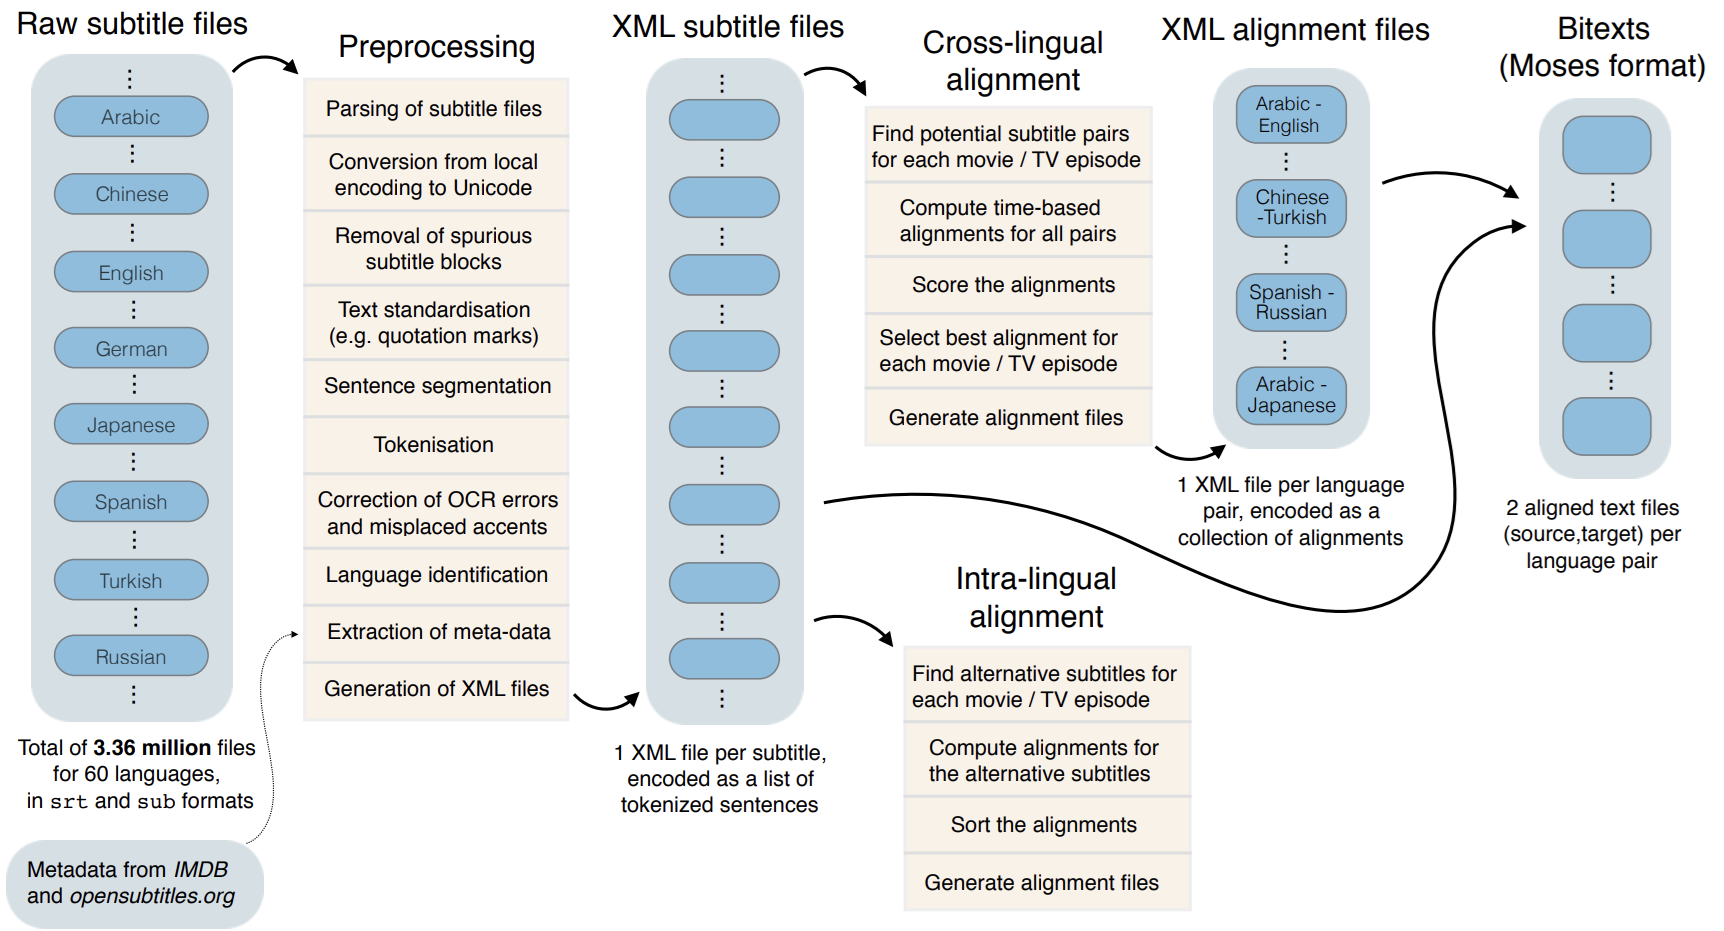
\includegraphics[width=\textwidth]{opensubs_corpus_processing.png}
	\caption{Pre-processing of the OPUS OpenSubtitles parallel corpus.}
	\label{fig:opensubtitles-pipeline}
\end{figure}

The OPUS Subtitles dataset contains not only the parallel sentences, but also movie identifiers from the Internet Movie Database (\textit{IMDB}) \footnote{\url{https://www.imdb.com/}}, which enables us to reconstruct the title of the movie from whose script each sentence originates using the \texttt{imdby} Python package \footnote{\url{https://pypi.org/project/imdby/}}.
While the dataset contains entire subtitles, these are not appropriate input data for the NSP task, as film subtitles consist of dialogue instead of continuous text.
Our preliminary tests showed this, with our NSP model showing very low accuracy when given contiguous subtitle sentence pairs as inputs.

% creation of final data set
While the newest version of the OpenSubtitles dataset is \textit{v2024}, this version did not exist at the outset of this work
\footnote{\url{https://web.archive.org/web/20241110103141/https://opus.nlpl.eu/OpenSubtitles/corpus/version/OpenSubtitles}, last accessed on May 4, 2025.}.
Hence, the version employed in this work is \textit{v2018}.
Because of limitations both in processing time and processing power on our side, we chose the relatively small \textit{English-Vietnamese} corpus, containing subtitles from 3,864 subtitles in total.
While the corpus contains the lines for all of these subtitles in long, continuous files, we split the lines into individual movie subtitles by their IMDB identifiers.
Apart from this, no pre-processing was performed on the subtitles by us.

\subsubsection{Modeling of Language Contexts}
Unlike Wikipedia, the subtitles in the OPUS OpenSubtitles dataset are not tagged with categories comparable to Wikipedia articles.
While the IMDB identifier would allow grouping subtitles by movie genre, the usefulness of such a grouping to model smaller contexts is questionable, as the genre of a movie is not the same as a topic, and thus in our estimation less likely to have an influence on useful words in the movie script.
For this reason, we do not perform such a grouping.
Instead, for large context vocabulary list compilation with the OpenSubtitles dataset, we only model the context of movies in general, using a random sample of 632 subtitles from the dataset for this grouping.
The efficiency of the vocabulary lists generated on the basis of these subtitles are tested on another random set of 30 subtitles (disjoint with the generation dataset of 632 subtitles).
We also use single movie subtitles to model small contexts, where list is generated and evaluated on the same lines for each movie (similarly to the generation and evaluation of single Wikipedia articles).

\subsection{TF-IDF Background Corpus: Oscar} \label{sec:oscar}
For the implementation of TF-IDF, we require a generic background corpus to normalize raw word frequencies found in context-specific corpora (that is, to calculate the IDF part of TF-IDF).
For this purpose, corpora crawled from the internet offer themselves as an attractive option, as web content is diverse in that it encompassed both formal and informal content on many different topics.

We reject the Common Crawl and Wortschatz Leipzig datasets for the reasons already stated in Section \ref{sec:rejected-corpora}.
Instead, we use a corpus from the \textit{Oscar} project \cite{suarezAsynchronousPipelineProcessing2019} as a background corpus:
Each \textit{Oscar} corpus is a cleaned-up version of a \textit{Common Crawl} dataset, on which pre-processing steps such as HTML stripping and removal of boilerplate content have already been performed.
It consists of (whole) web pages, and most importantly, its content is language-tagged, covering more than 150 languages in total.
The corpus used is available on the \textit{HuggingFace} platform under the path \texttt{oscar-corpus/oscar} with the name \texttt{unshuffled\_deduplicated\_en} \footnote{\url{https://huggingface.co/datasets/oscar-corpus/oscar}, last accessed May 2, 2025.}.
Due to its vast size, we do not use the entire corpus, but a random sample of 53,178 documents from this dataset to calculate inverse document frequency.

\subsection{Final Data Set} \label{sec:final-dataset}
The previous sections have described the creation of the small and large context corpora which we use in our implementation to generate and evaluate lists of vocabulary.
This section briefly summarizes all of our final corpora to provide an overview of the data we work with and whose evaluation is shown in Chapter \ref{ch:evaluation}.

% We use two data sources to model linguistic contexts, i.e., Wikipedia articles and subtitles from the OPUS OpenSubtitles dataset.
% For both sources, we generate and evaluate lists for \textbf{small and large contexts}:
% In the \textbf{small context} scenario, we generate a vocabulary list from a single Wikipedia article or OPUS subtitle.
% We then evaluate the generated vocabulary list on the same corpus.
% This covers the intended use case where a learner wishes to read an article or watch a movie, and study the most important words beforehand.
%
% In the \textbf{large context} scenario, we generate the vocabulary list from a number of single corpora, grouped by context, and the set of single corpora used for generation evaluation is disjoint:
% For Wikipedia, we use 80\% of the articles in each of four Wikipedia categories to create a vocabulary list specific to that category, and evaluate the list on the remaining 20\% of the category's articles.
% For the OpenSubtitles dataset, a sample of 632 subtitles is used for generation and sample of 30 subtitles for evaluation.
% The large context scenario was created to test how useful the words given by each approach are to a learner who is trying to increase their general understanding of texts in a certain context, without knowing the exact texts before engaging with them.
To avoid repetitiousness in the following sections, we will call a single article or single subtitle a \textbf{single corpus}.
We can categorize our evaluation by two both the corpus source and the scale of the evaluation, giving us four categories:


\begin{enumerate}
	\item A single Wikipedia article, where the lines used for list generation and evaluation are the same.
	\item A single subtitle, where the lines used for list generation and evaluation are the same.
	\item A Wikipedia category, where vocabulary lists are generated on the 80\% of articles in that category, and evaluated on the 20\% article set.
	\item OPUS OpenSubtitles, using 632 subtitles for list generation and 30 for evaluation.
\end{enumerate}

This amounts to a total number of five large contexts modeled in this work:
Four Wikipedia categories and one general OpenSubtitles context.
Table \ref{tbl:train-test-corpora} shows the number of single corpora (articles or subtitles) in each composite corpus.

\begin{table}[ht]
	\centering
	\begin{tabular}{lrr}
\toprule
 & List generation & List evaluation \\
Composite Corpus &  &  \\
\midrule
1980s English-language films & 20 & 6 \\
20th-century American actresses & 44 & 11 \\
20th-century American male actors & 86 & 22 \\
World War II political leaders & 16 & 5 \\
OpenSubtitles & 632 & 30 \\
\bottomrule
\end{tabular}

	\caption{Number of single corpora in the generation and evaluation portions for each large context corpus.}
	\label{tbl:train-test-corpora}
\end{table}


To gain an understanding of the data, Table \ref{tbl:corpus-sizes} shows a few key metrics of each corpus type.
It can be seen that, while OpenSubtitles subtitles contain of more lines on average, the Wikipedia articles feature much longer sentences (over three times longer on average than the sentences in subtitles).
This makes sense, as Wikipedia articles are written in an academic style, while movie subtitles tend to be more informal.
Wikipedia articles also contain a higher number of unique words on average, despite containing a lower number of words in total.
This may hint at a higher diversity of vocabulary employed in articles, although a higher number of named entities may also contribute to the higher count of unique words.

\begin{table}[ht]
	\centering
	\resizebox{\textwidth}{!}{%
		\begin{tabular}{lrrrrr}
\toprule
 & Corpora & Avg. lines & Avg. words & Avg. unique words & Avg. words per line \\
Corpus Type &  &  &  &  &  \\
\midrule
Wikipedia article & 210 & 253 & 4382 & 1211 & 17.3 \\
OpenSubs subtitle & 632 & 901 & 5436 & 1050 & 6.0 \\
\bottomrule
\end{tabular}

	}
	\caption{General statistics on corpora, per corpus type.}
	\label{tbl:corpus-sizes}
\end{table}


For a more granular overview, we also show these metrics for individual categories in Table \ref{tbl:corpus-sizes-per-wiki-category}.
Most obvious is the fact that the articles of \textit{World War II political leaders} are, on average, much longer than those films or actors of either gender.
Another notable pattern is that the articles of male actors tend to be longer than those of their female counterparts.


\begin{table}[ht]
	\centering
	\resizebox{\textwidth}{!}{%
		\begin{tabular}{lrrrrr}
\toprule
 & \# Corpora & Lines & Words & Unique Words & Words per Line \\
Wikipedia Category &  &  &  &  &  \\
\midrule
1980s English-language films & 26 & 160 & 2950 & 1014 & 18.4 \\
20th-century American actresses & 55 & 188 & 3296 & 934 & 17.5 \\
20th-century American male actors & 108 & 245 & 4157 & 1180 & 17.0 \\
World War II political leaders & 21 & 575 & 10159 & 2340 & 17.7 \\
\bottomrule
\end{tabular}

	}
	\caption{General statistics on corpora, per Wikipedia article category.}
	\label{tbl:corpus-sizes-per-wiki-category}
\end{table}

\subsubsection{Construction of NSP Corpora}
As mentioned in Section \ref{sec:document-level-corpus}, the next sentence prediction task requires consecutive sentences in order to be performed.
Out of the two context-specific corpus types which we employ, only Wikipedia articles consist of such consecutive sentences.
This is confirmed by the fact that preliminary investigations showed that the NSP model's performance on OpenSubtitles corpora was essentially equal to that of random guessing.
Thus, the NSP task is only performed on Wikipedia articles.
The NSP corpus of an article is constructed by simply taking each consecutive sentence pair from the article.
We do not construct negative examples, for the reason that the words with the most impact on the performance of the model would be words that tell the model that two sentences are \textit{not} connected, which does not appear to us to be useful information.
In the next section, we introduce the XAI methods which we use, in combination with the NLP tasks, to find the most useful words in the corpora described in this chapter.

\section{XAI Methods} \label{sec:xai-methods}
In order to appraise the influence of words in a corpus on the performance of an AI model performing NLP tasks on it, this work employs Explainable AI methods, as explained in Section \ref{sec:xai-as-tools-of-analysis}.
This section first puts forth the desiderata for the XAI methods, and then presents our choices of methods.
Due to time constraints, we limited our research to relatively simple methods.
While we gained valuable insights with the methods presented in this chapter, we acknowledge that better results may be achievable by using XAI approaches with more robust research.

\subsection{Desiderata}
Section \ref{sec:explainable-ai} has introduced essential distinctions between XAI methods which help us determine which methods are appropriate for our purpose:
We employ local, feature attribution methods of both model-specific and model-agnostic type, as these allow use to gauge the importance of words in the input.
Model-specific methods have an advantage in terms of computational efficiency, as they generally require fewer model calls to attribute importances to features, instead leveraging the internal structure of a model to arrive at explanations.
On the other hand, model-agnostic methods are useful in that they can be used on any model, and in that they gauge the input-output relationship from empirical data, observing the way changes to the model input change its output.

There is another desideratum which we impose on our XAI methods:
The XAI method should allow the model to \textbf{process input sentences in their original sequential form}, and not only as a \textit{bag of words}:
Some methods, such as SHAP \cite{lundbergUnifiedApproachInterpreting2017} and LIME \cite{ribeiroWhyShouldTrust2016}, were originally developed for structured data with a fixed number of input features.
Therefore, they are restricted to analyzing models whose inputs are not sequential, but in the form of a vector indicating whether a particular word is present in the sentence, with no regard to the word order and thus of syntactic relations between words.
In our view, this is problematic, as this simplification of the input could lead the methods to attribute low importance to words such as "not", which only affect the meaning of a sentence in combination with its other words.
For this reason, we did not employ the popular XAI methods SHAP or LIME in this work.

In the following sections, we present three model-agnostic XAI methods, which we use in the implementation of our vocabulary list generation approach described in Section \ref{sec:list-generation}.
These function by perturbing the inputs to the model and analyzing the changes in output.
They differ in how the perturbation is performed:
Single Token Ablation removes single tokens from the inputs, whereas Single Token Summary works by setting the input to a single token.
The third method, Progressive Summary, attempts to find the most important words in sentences by iteratively building up the input sentence, one token at a time.
For each perturbed sentence, we then measure how close its model output is from to output for the unperturbed sentence.

For the NSP task, only the first sentence of the pair is perturbed.
Apart from reducing the number of model calls, this is because, for Single Token Summary, removing all words from both sentences except one would mean that one of the sentences would usually be empty, which does not seem to us to be an informative perturbation.
This has the consequence that the word lists generated with the NSP task do not include the words form the last line of each corpus, as it does not have a corresponding next sentence.

After the model-agnostic methods, we detail our use of the model-specific transformer attention approach mentioned in Section \ref{sec:transformer}, as it requires more post-processing than the model-agnostic methods.
The relationship of the XAI methods to the NLP tasks is also discussed, as not every combination of XAI method and NLP task is feasible, either because it requires an unrealistic amount of computation or because the results of the combination are difficult to evaluate.
The results of the experiments with these methods are presented in Chapter \ref{ch:evaluation}.


\subsection{Single Token Ablation}
Our aim in using XAI methods is to find out which words, if known, improve the model's performance the most, when compared to not knowing the word.
Perhaps the simplest way of testing this is by going through every word in the AI model's input, and examining the impact on model performance when the word is removed from the input.
Within this work, this approach is called \textbf{Single Token Ablation}.
We show an example of how we perform Single Token Ablation on an input datum can be seen in Figure \ref{fig:single-token-ablation-sentemb} for sentence embedding task, and Figure \ref{fig:single-token-ablation-nsp} for next sentence prediction.

\paragraph{Approach:}
For an input sentence, we run the model on the unmodified sentence to get a baseline performance.
We then get the unique words in the input by using the tokenizer and merging sub-word tokens back into words.
For BERT tokens, this merging is a simple process, as sub-tokens which are not at the beginning of a word start with \texttt{"\#\#"}(See Section \ref{sec:tokenization}).
For each word in the input, we create a variation of the input where the word is removed.
We then run the model on all variations and measure the performance.
The estimated utility in this approach is given by the difference in performance between the variation's performance and that of the baseline output, as a high distance between the outputs implies that the word is important to the sentence's meaning.

\paragraph{Critical Evaluation:}
One advantage of Single Token Ablation is its conceptual simplicity, as it is easy to implement.
Furthermore, its time complexity is fairly low for a feature method, as it requires only one model call for each unique token in the sentence ($\mathcal{O}(n)$).
Before running experiments, we anticipated that due to this simplicity, Single Token Ablation would not work well on long sentences, where leaving out a single token would not seem to have a great impact on the meaning of the sentence.
Furthermore, this method does not take into account the utility of a word in the context of word combinations.
However, among the methods used in this paper, this method generates lists which achieve some of the highest efficiencies results in the final evaluation, especially for large vocabulary sizes.

\begin{figure}[H]
	\begin{center}
	\scalebox{0.75}{
		\begin{tikzpicture}[node distance=1.8cm and 2.5cm, every node/.style={font=\small}]

			% Styles
			\tikzstyle{process} = [rectangle, rounded corners, minimum width=3.5cm, minimum height=1cm, text centered, draw=black, fill=blue!10, text width=8.5cm]
			\tikzstyle{arrow} = [thick, ->, >=Stealth]
			\tikzstyle{data} = [align=left, text width=8.5cm, anchor=west]

			% Process Nodes
			\node (n1) [process] {Input sentence};
			\node (n2) [process, below=of n1] {Tokenize};
			\node (n3) [process, below=of n2] {Merge tokens, filter named entities and special tokens};
			\node (n4) [process, below=2cm of n3] {Make sentence variations by ablating merged tokens};
			\node (n5) [process, below=3cm of n4] {Run model on baseline and variations };
			\node (n6) [process, below=of n5] {Calculate cosine distance between variation vectors and baseline};

			% Anchor point to align all data nodes horizontally
			\node (anchor) [right=of n1] {};

			% Data Nodes, all vertically stacked but aligned to 'anchor'
			\node (d1) [data] at (anchor) {\texttt{"Abraham Lincoln faced enmity in 1863."}};
			\node (d2) [data, right=of n2] {
			\texttt{['[CLS]', 'abraham', 'lincoln', 'faced', 'en', '\#\#mity', 'in', '1863', '.', '[SEP]']}
			};
			\node (d3) [data, right=of n3] { \texttt{['faced', 'enmity', 'in']} };
			\node (d4) [data, right=of n4] {
				\textbf{(Baseline):} \\
				\quad \texttt{"abraham lincoln faced enmity in 1863."}\\
				\textbf{faced:} \\
				\quad \texttt{"abraham lincoln enmity in 1863."}\\
				\textbf{enmity:} \\
				\quad 	\texttt{"abraham lincoln faced in 1863."}\\
				\textbf{in:} \\
				\quad \texttt{"abraham lincoln faced enmity 1863."}\\
			};
			\node (d5) [data, right=of n5] {
				\begin{tabular}{@{}ll@{}}
					\textbf{(Baseline):} & $\vec{r}$ \\
					\textbf{faced:}      & $\vec{a}$ \\
					\textbf{enmity:}     & $\vec{b}$ \\
					\textbf{in:}         & $\vec{c}$ \\
				\end{tabular}
			};
			\node (d6) [data, right=of n6] {
				\begin{tabular}{@{}ll@{}}
					\textbf{faced:}  & $\text{CosDist}(\vec{a}, \vec{r}) = \texttt{0.5}$ \\
					\textbf{enmity:} &  $\text{CosDist}(\vec{b}, \vec{r}) = \texttt{0.7}$ \\
					\textbf{in:}     &  $\text{CosDist}(\vec{c}, \vec{r}) = \texttt{0.3}$ \\
				\end{tabular}
			};

			% Arrows between process nodes (left column)
			\draw [arrow] (n1) -- (n2);
			\draw [arrow] (n2) -- (n3);
			\draw [arrow] (n3) -- (n4);
			\draw [arrow] (n4) -- (n5);
			\draw [arrow] (n5) -- (n6);

		\end{tikzpicture}
	}
\end{center}


	\caption{Example of Single Token Ablation with sentence embedding, on one sentence.}
	\label{fig:single-token-ablation-sentemb}
\end{figure}

\begin{figure}[H]
	\begin{center}
	\scalebox{0.75}{
		\begin{tikzpicture}[node distance=1.8cm and 2.5cm, every node/.style={font=\small}]

			% Styles
			\tikzstyle{process} = [rectangle, rounded corners, minimum width=3.5cm, minimum height=1cm, text centered, draw=black, fill=blue!10, text width=8.5cm]
			\tikzstyle{arrow} = [thick, ->, >=Stealth]
			\tikzstyle{data} = [align=left, text width=8.5cm, anchor=west]

			% Process Nodes
			\node (n1) [process] {Input sentence pair};
			\node (n2) [process, below=of n1] {Tokenize the first sentence};
			\node (n3) [process, below=of n2] {Merge tokens, filter named entities and special tokens};
			\node (n4) [process, below=3cm of n3] {Make sentence pair variations by ablating merged tokens from the first line};
			\node (n5) [process, below=4cm of n4] {Run model for variations, predicting $p_{is\_next}$};
			\node (n6) [process, below=of n5] {Calculate word utility by $|p_{baseline} - p_{w}|$};

			% Anchor point to align all data nodes horizontally
			\node (anchor) [right=of n1] {};

			% Data Nodes, all vertically stacked but aligned to 'anchor'
			\node (d1) [data] at (anchor) {\texttt{["Abraham Lincoln faced enmity in 1863."\\
								"Yet, he prevailed in the end."]}};
			\node (d2) [data, right=of n2] {
			\texttt{['[CLS]', 'abraham', 'lincoln', 'faced', 'en', '\#\#mity', 'in', '1863', '.', '[SEP]']}
			};
			\node (d3) [data, right=of n3] { \texttt{['faced', 'enmity', 'in'] }};
			\node (d4) [data, right=of n4] {
				\textbf{(Baseline):}  \\
				\quad 	\texttt{["abraham lincoln faced enmity in 1863.",\\
							\quad 		"yet, he prevailed in the end."] }\\
				\textbf{faced:}  \\
				\quad 	\texttt{["abraham lincoln enmity in 1863.",\\
							\quad 		"yet, he prevailed in the end."] }\\
				\textbf{enmity:}   \\
				\quad 	\texttt{["abraham lincoln faced in 1863.", \\
							\quad 			"yet, he prevailed in the end."] }\\
				\textbf{in:}\\
				\quad 	\texttt{["abraham lincoln faced enmity 1863.",\\
							\quad 				"yet, he prevailed in the end."] }\\
			};
			\node (d5) [data, right=of n5] {
				\begin{tabular}{@{}ll@{}}
					\textbf{(Baseline):} & \texttt{0.9} \\
					\textbf{faced:}      & \texttt{0.5} \\
					\textbf{enmity:}     & \texttt{0.3} \\
					\textbf{in:}         & \texttt{0.7} \\
				\end{tabular}

			};
			\node (d6) [data, right=of n6] {
				\begin{tabular}{@{}ll@{}}
					\textbf{faced:} & \texttt{0.4}  \\
					\textbf{enmity:} & \texttt{0.6} \\
					\textbf{in:} & \texttt{0.2}     \\
				\end{tabular}
			};

			% Arrows between process nodes (left column)
			\draw [arrow] (n1) -- (n2);
			\draw [arrow] (n2) -- (n3);
			\draw [arrow] (n3) -- (n4);
			\draw [arrow] (n4) -- (n5);
			\draw [arrow] (n5) -- (n6);

		\end{tikzpicture}
	}
\end{center}

	\caption{Example of Single Token Ablation with next sentence prediction, on one sentence pair.}
	\label{fig:single-token-ablation-nsp}
\end{figure}

\subsection{Single Token Summary} \label{sec:single-token-summary}
The second feature model-agnostic method can be seen as the opposite of Single Token Ablation:
Instead of taking out one word at a time, we use as input only a single word at a time (apart from named entities and punctuation, which are always present).
Because the intention behind this method is finding words which, on their own, carry much of the meaning of a sentence, we call it \textbf{Single Token Summary}.
Examples of its use are shown in Figure \ref{fig:single-token-summary-sentemb} and \ref{fig:single-token-summary-nsp}.

\paragraph{Approach:}
We first run the model on an "empty" variation of the input sentence where only punctuation and named entities are included, using its output as the starting performance.
We then decompose the input sentence into its word tokens.
For each word, a variation of the sentence is put through the model where, in addition to punctuation and named entities, only that word appears.
The utility in this approach is calculated by taking the performance improvement of a word's sentence variation compared to the performance of the "empty" sentence.

\paragraph{Critical Evaluation:}
Like Single Token Ablation, this method requires only one model call for each unique token in the sentence ($\mathcal{O}(n)$).
One of the motivations behind this method was to find tokens helpful to beginners more efficiently, as it attempts to reconstruct the meaning of each sentence with a minimal vocabulary.
Our evaluation found that, in general, this method produces vocabulary lists with high efficiency at low vocabulary sizes, confirming the theory that it prioritizes words that would be useful to learn for beginners.

\begin{figure}[H]
	\begin{center}
	\scalebox{0.75}{
		\begin{tikzpicture}[node distance=1.8cm and 2.5cm, every node/.style={font=\small}]

			% Styles
			\tikzstyle{process} = [rectangle, rounded corners, minimum width=3.5cm, minimum height=1cm, text centered, draw=black, fill=blue!10, text width=8.5cm]
			\tikzstyle{arrow} = [thick, ->, >=Stealth]
			\tikzstyle{data} = [align=left, text width=8.5cm, anchor=west]

			% Process Nodes
			\node (n1) [process] {Input sentence};
			\node (n2) [process, below=of n1] {Tokenize};
			\node (n3) [process, below=of n2] {Merge tokens, filter named entities and special tokens};
			\node (n4) [process, below=2cm of n3] {Make sentence variations by inserting merged tokens into "empty" sentence};
			\node (n5) [process, below=3cm of n4] {Run model on "empty" sentence, baseline, and variations };
			\node (n6) [process, below=of n5] {Calculate word utility by how much closer the vector gets to the baseline, compared to the empty input};

			% Anchor point to align all data nodes horizontally
			\node (anchor) [right=of n1] {};

			% Data Nodes, all vertically stacked but aligned to 'anchor'
			\node (d1) [data] at (anchor) {\texttt{"Abraham Lincoln faced enmity in 1863."}};
			\node (d2) [data, right=of n2] {
			\texttt{['[CLS]', 'abraham', 'lincoln', 'faced', 'en', '\#\#mity', 'in', '1863', '.', '[SEP]']}
			};
			\node (d3) [data, right=of n3] { \texttt{['faced', 'enmity', 'in']} };
			\node (d4) [data, right=of n4] {
				\textbf{(Empty):} \\
				\quad \texttt{"abraham lincoln 1863."}\\
				\textbf{(Baseline):} \\
				\quad \texttt{"abraham lincoln faced enmity in 1863."}\\
				\textbf{faced:} \\
				\quad \texttt{"abraham lincoln faced 1863."}\\
				\textbf{enmity:} \\
				\quad 	\texttt{"abraham lincoln enmity 1863."}\\
				\textbf{in:} \\
				\quad \texttt{"abraham lincoln in 1863."}\\
			};
			\node (d5) [data, right=of n5] {
				\begin{tabular}{@{}ll@{}}
					\textbf{(Empty):}    & $\vec{e}$ \\
					\textbf{(Baseline):} & $\vec{r}$ \\
					\textbf{faced:}    & $\vec{a}$ \\
					\textbf{enmity:}   & $\vec{b}$ \\
					\textbf{in:}       & $\vec{c}$ \\
				\end{tabular}
			};
			\node (d6) [data, right=of n6] {
\begin{tabular}{@{}ll@{}}
        \textbf{faced:}  & $\text{CosDist}(\vec{e}, \vec{r}) - \text{CosDist}(\vec{a}, \vec{r})= \texttt{0.5}$ \\
        \textbf{enmity:} & $\text{CosDist}(\vec{e}, \vec{r}) - \text{CosDist}(\vec{b}, \vec{r})= \texttt{0.7}$ \\
        \textbf{in:}     & $\text{CosDist}(\vec{e}, \vec{r}) - \text{CosDist}(\vec{c}, \vec{r})= \texttt{0.3}$ \\
    \end{tabular}
			};

			% Arrows between process nodes (left column)
			\draw [arrow] (n1) -- (n2);
			\draw [arrow] (n2) -- (n3);
			\draw [arrow] (n3) -- (n4);
			\draw [arrow] (n4) -- (n5);
			\draw [arrow] (n5) -- (n6);

		\end{tikzpicture}
	}
\end{center}


	\caption{Example of Single Token Summary with sentence embedding, on one line.}
	\label{fig:single-token-summary-sentemb}
\end{figure}

\begin{figure}[H]
	\begin{center}
	\scalebox{0.75}{
		\begin{tikzpicture}[node distance=1.8cm and 2.5cm, every node/.style={font=\small}]

			% Styles
			\tikzstyle{process} = [rectangle, rounded corners, minimum width=3.5cm, minimum height=1cm, text centered, draw=black, fill=blue!10, text width=8.5cm]
			\tikzstyle{arrow} = [thick, ->, >=Stealth]
			\tikzstyle{data} = [align=left, text width=8.5cm, anchor=west]

			% Process Nodes
			\node (n1) [process] {Input sentence pair};
			\node (n2) [process, below=of n1] {Tokenize the first sentence};
			\node (n3) [process, below=of n2] {Merge tokens, filter named entities and special tokens};
			\node (n4) [process, below=4cm of n3] {Run model on "empty" sentence, baseline, and variations };
			\node (n5) [process, below=5cm of n4] {Run model for variations, predicting $p_{is\_next}$};
			\node (n6) [process, below=of n5] {Calculate word utility by \\
			$||(p_{baseline} - p_{empty})| - |(p_{baseline} - p_{word})||$};

			% Anchor point to align all data nodes horizontally
			\node (anchor) [right=of n1] {};

			% Data Nodes, all vertically stacked but aligned to 'anchor'
			\node (d1) [data] at (anchor) {\texttt{["Abraham Lincoln faced enmity in 1863."\\
								"Yet, he prevailed in the end."]}};
			\node (d2) [data, right=of n2] {
			\texttt{['[CLS]', 'abraham', 'lincoln', 'faced', 'en', '\#\#mity', 'in', '1863', '.', '[SEP]']}
			};
			\node (d3) [data, right=of n3] { \texttt{['faced', 'enmity', 'in'] }};
			\node (d4) [data, right=of n4] {
				\textbf{(Empty):}  \\
				\quad 	\texttt{["abraham lincoln 1863.",\\
							\quad 		"yet, he prevailed in the end."] }\\
				\textbf{(Baseline):}  \\
				\quad 	\texttt{["abraham lincoln faced enmity in 1863.",\\
							\quad 		"yet, he prevailed in the end."] }\\
				\textbf{faced:}  \\
				\quad 	\texttt{["abraham lincoln faced 1863.",\\
							\quad 		"yet, he prevailed in the end."] }\\
				\textbf{enmity:}   \\
				\quad 	\texttt{["abraham lincoln enmity 1863.", \\
							\quad 			"yet, he prevailed in the end."] }\\
				\textbf{in:}\\
				\quad 	\texttt{["abraham lincoln in 1863.",\\
							\quad 				"yet, he prevailed in the end."] }\\
			};
			\node (d5) [data, right=of n5] {
				\begin{tabular}{@{}ll@{}}
					\textbf{(Empty):} & \texttt{0.4} \\
					\textbf{(Baseline):} & \texttt{0.9} \\
					\textbf{faced:}      & \texttt{0.6} \\
					\textbf{enmity:}     & \texttt{0.8} \\
					\textbf{in:}         & \texttt{0.5} \\
				\end{tabular}

			};
			\node (d6) [data, right=of n6] {
				\begin{tabular}{@{}ll@{}}
					\textbf{faced:} & \texttt{0.2}  \\
					\textbf{enmity:} & \texttt{0.4} \\
					\textbf{in:} & \texttt{0.1}     \\
				\end{tabular}
			};

			% Arrows between process nodes (left column)
			\draw [arrow] (n1) -- (n2);
			\draw [arrow] (n2) -- (n3);
			\draw [arrow] (n3) -- (n4);
			\draw [arrow] (n4) -- (n5);
			\draw [arrow] (n5) -- (n6);

		\end{tikzpicture}
	}
\end{center}

	\caption{Example of Single Token Summary with next sentence prediction, on one sentence pair.}
	\label{fig:single-token-summary-nsp}
\end{figure}

% \paragraph{Compatibility with NLP tasks:}
% \todo{compat with NSP?}

\subsection{Progressive Summary} \label{sec:progressive-summary}
While Single Token Summary is easy to implement and computationally inexpensive, it has the conceptual disadvantage of not taking into account the utility of word combinations.
To achieve a more accurate evaluation, we present another "summary" approach, where the sentence is built up one word at a time.
The progressive building up of the sentence is meant to give the best order to learn words in for a single line, starting from the point of a simulated learner who does not know any words.
For this reason, we only perform the "progressive" approach building up the sentence, but do not attempt the reverse, i.e., ablating one word after another from a sentence.
We call this approach "Progressive Summary".
Because this approach is much more computationally intensive and our next sentence prediction model takes more calculation time than our sentence embedding model (see Section \ref{sec:eval-speed}), we did not use Progressive Summary in combination with the NSP task.
An example of this method (with sentence embedding) is shown in Figure \ref{fig:progressive-summary}.

\paragraph{Approach:}
For an input sentence, this approach starts the same as Single Token Summary, by checking the performance of the one-word sentence variations.
We then use the word with the highest improvement in the next iteration:
From the other words in the sentence, we check which one improves the performance the most when used in addition to our already found word.
By iterating this method for the remaining words, we progressively reconstruct the original sentence, which each step adding the word which brings the output closest to the output of the unperturbed baseline.
The estimated utility of a word is the boost in performance which is brought to the sentence when the word is added.

\begin{figure}[H]
	\begin{center}
	\scalebox{0.75}{
		\begin{tikzpicture}[node distance=1.8cm and 2.5cm, every node/.style={font=\small}]

			% Styles
			\tikzstyle{process} = [rectangle, rounded corners, minimum width=3.5cm, minimum height=1cm, text centered, draw=black, fill=blue!10, text width=8.5cm]
			\tikzstyle{arrow} = [thick, ->, >=Stealth]
			\tikzstyle{data} = [align=left, text width=8.5cm, anchor=west]

			% Process Nodes
			\node (n1) [process] {Input sentence};
			\node (n2) [process, below=of n1] {Tokenize};
			\node (n3) [process, below=of n2] {Merge tokens, filter named entities and special tokens};
			\node (n4) [process, below=2cm of n3] {Make "baseline" sentence to evaluate performance", and "empty" sentence to start the summary};
			\node (n5) [process, below=5cm of n4] {For each word, run the model on its variation, evaluate the outputs, and pick the next best word to add to the summary};
			\node (n6) [process, below=5cm of n5] {Repeat for remaining words};
			\node (n7) [process, below=5cm of n6] {Repeat for remaining words};
			\node (n8) [process, below=3cm of n7] {Return word utilities};

			% Anchor point to align all data nodes horizontally
			\node (anchor) [right=of n1] {};

			% Data Nodes, all vertically stacked but aligned to 'anchor'
			\node (d1) [data] at (anchor) {\texttt{"Abraham Lincoln faced enmity in 1863."}};
			\node (d2) [data, right=of n2] {
			\texttt{['[CLS]', 'abraham', 'lincoln', 'faced', 'en', '\#\#mity', 'in', '1863', '.', '[SEP]']}
			};
			\node (d3) [data, right=of n3] { \texttt{['faced', 'enmity', 'in']} };
			\node (d4) [data, right=of n4] {
				\textbf{(Empty):} \\
				\quad \texttt{"abraham lincoln 1863."}\\
				\textbf{(Baseline):} \\
				\quad \texttt{"abraham lincoln faced enmity in 1863."}\\
				Current sentence: \\
				\quad \texttt{"abraham lincoln 1863."}\\
				Current performance: \texttt{0.4}\\
			};
			\node (d5) [data, right=of n5] {
				Remaining words: \texttt{['faced', 'enmity', 'in']} \\
				\quad \textbf{faced:} \\
				\mbox{\quad \quad \texttt{"abraham lincoln faced 1863."} $\rightarrow$ \texttt{0.6} }\\
				\quad \textbf{enmity:} \\
				\mbox{\quad \quad 	\texttt{"abraham lincoln enmity 1863."} $\rightarrow$ \texttt{0.7}}\\
				\quad \textbf{in:} \\
				\mbox{\quad \quad \texttt{"abraham lincoln in 1863."} $\rightarrow$ \texttt{0.5}}\\
				Next best word: \textbf{enmity}\\
				Utility of \textbf{enmity}: $0.7 - 0.4 = 0.3$ \\
				Current sentence:  \\ 
				\quad \texttt{"abraham lincoln enmity 1863."}\\
				Current performance: \texttt{0.7}\\
			};
			\node (d6) [data, right=of n6] {
				Remaining words: \texttt{['faced', 'in']} \\
				\quad \textbf{faced:} \\
				\mbox{\quad \quad \texttt{"abraham lincoln faced enmity 1863." $\rightarrow$ 0.9} }\\
				\quad \textbf{in:} \\
				\mbox{\quad \quad \texttt{"abraham lincoln enmity in 1863." $\rightarrow$ 0.8}} \\
				Next best word: \textbf{faced}\\
				Utility of \textbf{faced}: $0.9 - 0.7 = 0.2$ \\
				Current sentence: \\
				\quad \texttt{"abraham lincoln faced enmity 1863."}\\

				Current performance: \texttt{0.9}\\
			};
			\node (d7) [data, right=of n7] {
				Remaining words: \texttt{['in']} \\
				\quad \textbf{in:} \\
				\mbox{\quad \quad \texttt{"abraham lincoln faced enmity in 1863."}$\rightarrow$ \texttt{1} }\\
				Next best word: \textbf{in}\\
			Utility of \textbf{in}: $1 - 0.9 = 0.1$ \\
				Current sentence:\\ 
				\quad \texttt{"abraham lincoln faced enmity in 1863."}\\
				Current performance: \texttt{1}\\
			};
			\node (d8) [data, right=of n8] {
				\begin{tabular}{@{}ll@{}}
					\textbf{faced:}  & \texttt{0.2} \\
					\textbf{enmity:} & \texttt{0.3} \\
					\textbf{in:}     & \texttt{0.1} \\
				\end{tabular}
			};

			% Arrows between process nodes (left column)
			\draw [arrow] (n1) -- (n2);
			\draw [arrow] (n2) -- (n3);
			\draw [arrow] (n3) -- (n4);
			\draw [arrow] (n4) -- (n5);
			\draw [arrow] (n5) -- (n6);
			\draw [arrow] (n6) -- (n7);
			\draw [arrow] (n7) -- (n8);

		\end{tikzpicture}
	}
\end{center}



	\caption{Example of Progressive Summary with sentence embedding, on one sentence.}
	\label{fig:progressive-summary}
\end{figure}

\paragraph{Critical Evaluation:}
For a single sentence, Progressive Summary would appear to be the most accurate in ordering its words by utility, as it considers the utility of each word in combination with the words which have already been found to be useful.
However, Progressive Summary is much more computationally intensive than Single Token Summary, which requires only one model call per word in the sentence.
Because of its iterative approach, for a sentence with 10 words, Progressive Summary calls the model $10+9+8+... = \sum_{i=1}^{n}i = \frac{n^2 + n}{2}$ times, which is a time complexity of $\mathcal{O}(n^2)$.
The fact that the word utilities are calculated in the context of the already included words also makes it difficult to judge how the results of Progressive Summary should be aggregated across lines.
Perhaps because of this difficulty, Progressive Summary did not outperform the simpler methods in our evaluation.


\subsection{Attention as Explanation}
The model-agnostic methods so far can be employed on any AI model.
However, as many of the latest state-of-the-art AI models follow the Neural Network architecture, and more specifically the transformer architecture (see Section \ref{sec:transformer}), we also attempt word utility estimation with a method specific to these models, namely attention.
% These model-specific XAI methods have the advantage of being computationally efficient:
% Model-agnostic methods extract information about the model by perturbing its inputs and analyzing the resulting changes in the output.
% This requires many model calls for one input datum.
% In contrast, model-specific methods can analyze the input-output relationship with only one model call, as they look into the model itself for information.
% We therefore try two model-specific methods for analyzing word utility as well, as their more efficient calculations means they can process more input data in a given time, which should increase the accuracy of the resulting word list for large corpora.
As stated before, transformer models use self-attention to assign importance to the connections between tokens in the input (if their input is in text format).
This may be used as a kind of explanation, as words which have strong connections to many other words in the sentence presumably are more important to the AI model's understanding of it than those receiving less self-attention.
Preliminary tests showed both of our chosen models producing very similar lists with attention, and so we only use this method in combination with our more time-efficient sentence embedding model. 
An example of an input line being processed with this approach is shown in Figure \ref{fig:attention}.

\paragraph{Approach:}
A transformer model is run with one line as input.
The transformer outputs a three-dimensional attention tensor, which attributes a value to each combination of attention head and pair of (sub-word) tokens in the input (this includes special tokens from the tokenizer, such as \texttt{[SEP]}, and punctuation).
We then aggregate the attention value of each token by summing over the attention heads, as well as one of the remaining axes of the attention tensor, resulting in one scalar value per (non-unique) token in the input.
Then, we again filter special tokens, punctuation and named entities, and merge sub-word tokens into words.
Next, the attention over all occurrences of each unique token is summed over, yielding one scalar attention for each unique word.
Finally, we normalize the attentions such that the total attention for all words in the line sums up to one.
The attributed attention to a word thus determines its estimated utility.

\begin{figure}[H]
	\begin{center}
	\scalebox{0.75}{
		\begin{tikzpicture}[node distance=1.8cm and 2.5cm, every node/.style={font=\small}]

			% Styles
			\tikzstyle{process} = [rectangle, rounded corners, minimum width=3.5cm, minimum height=1cm, text centered, draw=black, fill=blue!10, text width=8.5cm]
			\tikzstyle{arrow} = [thick, ->, >=Stealth]
			\tikzstyle{data} = [align=left, text width=8.5cm, anchor=west]

			% Process Nodes
			\node (n1) [process] {Input sentence};
			\node (n2) [process, below=of n1] {Tokenize the sentence};
			\node (n3) [process, below=3cm of n2] {Run the models and sum over the attentions for each token};
			\node (n4) [process, below=3cm of n3] {Filter special tokens, punctuation, and named entities, then merge the remaining sub-word tokens};
			\node (n5) [process, below=of n4] {Normalize the attention sum to 1};

			% Anchor point to align all data nodes horizontally
			\node (anchor) [right=of n1] {};

			% Data Nodes, all vertically stacked but aligned to 'anchor'
			\node (d1) [data] at (anchor) {\texttt{["Abraham Lincoln faced enmity in 1863."\\
								"Yet, he prevailed in the end."]}};
			\node (d2) [data, right=of n2] {
			\texttt{['[CLS]', 'abraham', 'lincoln', 'faced', 'en', '\#\#mity', 'in', '1863', '.', '[SEP]']}
			};
			\node (d3) [data, right=of n3] {
				\begin{tabular}{@{}ll@{}}
					\texttt{[CLS]}    & 400 \\
					\texttt{abraham}  & 300 \\
					\texttt{lincoln}  & 200 \\
					\texttt{faced}    & 150 \\
					\texttt{en}       & 150 \\
					\texttt{\#\#mity} & 200 \\
					\texttt{in}       & 100 \\
					\texttt{1863}     & 200 \\
					\texttt{.}        & 50  \\
					\texttt{[SEP]}    & 500 \\
				\end{tabular}
			};

			\node (d4) [data, right=of n4] {
				\begin{tabular}{@{}ll@{}}
					\texttt{faced}    & 150 \\
					\texttt{enmity}       & 350 \\
					\texttt{in}       & 100 \\
				\end{tabular}
			};
			\node (d5) [data, right=of n5] {
				\begin{tabular}{@{}ll@{}}
					\texttt{faced}    & 0.25 \\
					\texttt{enmity}       & 0.58 \\
					\texttt{in}       & 0.16 \\
				\end{tabular}
			};

			% Arrows between process nodes (left column)
			\draw [arrow] (n1) -- (n2);
			\draw [arrow] (n2) -- (n3);
			\draw [arrow] (n3) -- (n4);
			\draw [arrow] (n4) -- (n5);

		\end{tikzpicture}
	}
\end{center}


	\caption{Example of attention as explanation, on one sentence.}
	\label{fig:attention}
\end{figure}

\paragraph{Critical Evaluation:}
The main upshot of attention is that, as hinted at before, this method uses only one model call for one input line, and thus has a time complexity of $\mathcal{O}(1)$.
An important difference to the model-agnostic methods is that we do not control word masking with a tokenizer \textit{independent of the model}, thus the splitting of words is not under our direct control.
This can be an issue because it means that lists generated with the model-specific tokenizer are not necessarily comparable to lists from model-agnostic methods, as the word boundaries may differ between the lists.
However, we use the attention approach to explanation in combination with our sentence embedding model \texttt{all-MiniLM-L6-v2}, which uses a BERT tokenizer available under the same name on the \textit{HuggingFace} platform \footnote{\url{https://huggingface.co/sentence-transformers/all-MiniLM-L6-v2}}.
To the best of our knowledge, this tokenizer splits texts into the same tokens as the \texttt{bert-base-uncased} tokenizer which we use for token splitting in the model-agnostic methods, which should prevent such issues from arising.

In addition to this technical downside, attention is controversial as a mechanism to explain model decisions:
One point of critique is that, while attention influences the model's behavior, it is not a faithful explanation because alternative attention distributions can yield similar model outputs \cite{jainAttentionNotExplanation2019}.
On the other hand, it has been argued that the mere fact that a model chooses a particular attention distribution, rather than another, means that the actually generated distribution is a more plausible explanation than artificial adversarial distributions \cite{wiegreffeAttentionNotNot2019}.
As we will show in our list evaluation, when used with our list generation approach, attention produces vocabulary lists that are close in efficiency to those produced by the model-agnostic methods.
\todo{check the previous claim about the performance}


\section{Summary of the Implementation} \label{sec:implementation-final}
The previous chapters have argued for the choice of components in our theoretical approach to vocabulary list generation and evaluation.
This final section summarizes our implementation, which will be evaluated in the next chapter.
Section \ref{sec:impl-summary-description} describes the interaction of our selected components to the list generation approach, whereas Section \ref{sec:supported-languages} gives an overview of the supported languages of our implementation resulting from this setup.

\subsection{Interaction of Components} \label{sec:impl-summary-description}
We use two sources of corpora to model linguistic contexts, namely Wikipedia and the OPUS OpenSubtitles dataset.
From these, we create vocabulary lists for small and large contexts:
The small context lists are generated by running combinations of NLP tasks and XAI method on single corpora (single articles or single subtitles) from these sources.
The utility of a word for a given single corpus is calculated by taking the sum of the word's utility across all lines in the corpus.
For the large context scenario, we aggregate the utilities across the single corpora inside it:
In order to make short and long single corpora contribute equally to the final list, we sum across the corpus utilities, but normalize the total utility each corpus contributes to 1.

From Wikipedia, articles from four categories are used, both as the sources of single corpora and as large context corpora:
\textit{20th-century American actresses},
\textit{20th-century American male actors},
\textit{1980s English-language films}, and
\textit{World War II political leaders}.
For the OpenSubtitles subtitles, no such categorical division is trivially possible, and thus our large context consists simply of a large sample of subtitles from this dataset.

For \textbf{Wikipedia} articles, we use the following combinations of XAI method and NLP task to compile vocabulary lists:

\begin{table}[H]
	\centering
	\begin{tabularx}{\textwidth}{|X|X|}
		\hline
		\textbf{XAI Method}   & \textbf{Task}            \\
		\hline
		Single Token Ablation & Sentence embedding       \\
		\hline
		Single Token Ablation & Next sentence prediction \\
		\hline
		Single Token Summary  & Sentence embedding       \\
		\hline
		Single Token Summary  & Next sentence prediction \\
		\hline
		Progressive Summary   & Sentence embedding       \\
		\hline
		Attention             & Sentence embedding       \\
		\hline
	\end{tabularx}
\end{table}

For the subtitles from the \textbf{OPUS OpenSubtitles} dataset, we do not use the NSP task, as the AI model is not suited to be used with these lines.
This leaves the following combinations:

\begin{table}[H]
	\centering
	\begin{tabularx}{\textwidth}{|X|X|}
		\hline
		\textbf{XAI Method}   & \textbf{Task}      \\
		\hline
		Single Token Ablation & Sentence embedding \\
		\hline
		Single Token Summary  & Sentence embedding \\
		\hline
		Progressive Summary   & Sentence embedding \\
		\hline
		Attention             & Sentence embedding \\
		\hline
	\end{tabularx}
\end{table}



% \begin{figure}[H]
% 	\begin{center}
	\scalebox{0.75}{
		\begin{tikzpicture}[node distance=1.8cm and 2.5cm, every node/.style={font=\small}]

			% Styles
			\tikzstyle{process} = [rectangle, rounded corners, minimum width=3.5cm, minimum height=1cm, text centered, draw=black, fill=blue!10, text width=8.5cm]
			\tikzstyle{arrow} = [thick, ->, >=Stealth]
			\tikzstyle{data} = [align=left, text width=8.5cm, anchor=west]

			% Process Nodes
			\node (n1) [process] {Input sentence};
			\node (n2) [process, below=of n1] {Tokenize};
			\node (n3) [process, below=of n2] {Merge tokens, filter named entities and special tokens};
			\node (n4) [process, below=of n3] {Make sentence variations by ablating merged tokens};
			\node (n5) [process, below=of n4] {Run model for variations, evaluate performances};
			\node (n6) [process, below=of n5] {Calculate difference to baseline in performance};

			% Anchor point to align all data nodes horizontally
			\node (anchor) [right=of n1] {};

			% Data Nodes, all vertically stacked but aligned to 'anchor'
			\node (d1) [data] at (anchor) {\textbf{Baseline}: "Abraham Lincoln faced enmity in 1863."\\
				\textbf{Variation}: "Abraham Lincoln enmity 1863."
			};
			\node (d2) [data, right=of n2] {
			['[CLS]', 'abraham', 'lincoln', 'faced', 'en', '\#\#mity', 'in', '1863', '.', '[SEP]']
			};
			\node (d3) [data, right=of n3] { ['faced', 'enmity', 'in'] };
			\node (d4) [data, right=of n4] {
				\textbf{Baseline:} "abraham lincoln faced enmity in 1863."\\
				\textbf{faced:} "abraham lincoln enmity in 1863."\\
				\textbf{enmity:} "abraham lincoln faced in 1863."\\
				\textbf{in:} "abraham lincoln faced enmity 1863."\\
			};
			\node (d5) [data, right=of n5] {
				\textbf{Baseline:} 0.8\\
				\textbf{faced:} 0.5\\
				\textbf{enmity:} 0.3\\
				\textbf{in:} 0.7\\
			};
			\node (d6) [data, right=of n6] {
				[('faced', 0.3), ('enmity', 0.5), ('in', 0.1)]
			};

			% Arrows between process nodes (left column)
			\draw [arrow] (n1) -- (n2);
			\draw [arrow] (n2) -- (n3);
			\draw [arrow] (n3) -- (n4);
			\draw [arrow] (n4) -- (n5);
			\draw [arrow] (n5) -- (n6);

		\end{tikzpicture}
	}
\end{center}


% 	\caption{Example of sentence embedding scoring}
% 	\label{fig:list-evaluation-diagram}
% \end{figure}

\subsection{Supported Languages} \label{sec:supported-languages}
Our data pipeline contains various language-specific components, all of which must support a language in order for our approach to support vocabulary list generation in the language.
Table \ref{table:supported-languages} summarizes the theoretical language support of each component, including pre-processing.
As mentioned before, we use monolingual AI models in our implementation, but chose such models for which multilingual variants exist also (see Sections \ref{sec:nsp} and \ref{sec:sentence-embedding}), which is why, in the table, we show these variants instead of the multilingual ones.

{
\renewcommand{\arraystretch}{1.5}  % Increase the vertical padding for this table only
\begin{table}[H]
	\centering
	\begin{tabularx}{\textwidth}{|X|X|X|}
		\hline
		\textbf{Component}                          & \textbf{Supported Languages} & \textbf{Notes}                                                                                                                                                                                                                             \\
		\hline
		Tokenization                                & 104                          & Using the \texttt{bert-base-uncased} model\footnotemark[1].                                                                                                                                                                                 \\
		\hline
		Named Entity Recognition                    & 9                            & Using the \textit{spacy} model \texttt{xx\_ent\_wiki\_sm}\footnotemark[2]. The number of supported languages is not stated for this model, but it was trained on the \texttt{WikiNER} dataset\footnotemark[3], which contains 9 languages. \\
		\hline
		Next sentence prediction                    & 104                          & Using the \texttt{bert-base-multilingual-cased} model\footnotemark[4]                                                                                                                                                                      \\
		\hline
		Sentence Embedding                          & $>50$                        & Using the \texttt{paraphrase-multilingual-MiniLM-L12-v2} model\footnotemark[5].                                                                                                                                                             \\
		\hline
		Sentence splitting (for Wikipedia articles) & $>150$                       & Using the \texttt{xx\_sent\_ud\_sm} model\footnotemark[6], based on the \textit{Universal Dependencies} framework\footnotemark[7], which supports $>150$ languages.                                                                        \\
		\hline
		Filtering of Wikipedia sections             & (manual)                     & See Section \ref{sec:wikipedia-preprocessing}.                                                                                                                                                                                              \\
		\hline
		Wikipedia Corpus                            & $>300$                       & As of 2025, there exist Wikipedias in over 300 languages\footnotemark[8].                                                                                                                                                                   \\
		\hline
		OPUS OpenSubtitles Corpus                   & 94                           & See the corpus' website \footnotemark[9].                                                                                                                                                                                                                       \\
		\hline
	\end{tabularx}



	\caption{Languages supported by each component in the pipeline.}
	\label{table:supported-languages}
\end{table}
}

\footnotetext[1]{\url{https://huggingface.co/google-bert/bert-base-uncased}}
\footnotetext[2]{\url{https://spacy.io/models/xx\#xx_ent_wiki_sm}}
\footnotetext[3]{\url{https://huggingface.co/datasets/mnaguib/WikiNER}}
\footnotetext[4]{\url{https://huggingface.co/google-bert/bert-base-multilingual-cased}}
\footnotetext[5]{\url{https://www.sbert.net/docs/sentence_transformer/pretrained_models.html\#original-models}}
\footnotetext[6]{\url{https://spacy.io/models/xx\#xx_sent_ud_sm}}
\footnotetext[7]{\url{https://universaldependencies.org/}}
\footnotetext[8]{\url{https://en.wikipedia.org/wiki/List_of_Wikipedias}}
\footnotetext[9]{\url{https://opus.nlpl.eu/OpenSubtitles/corpus/version/OpenSubtitles}}

It can be seen that, apart from the manual selection of certain Wikipedia headings, named entity recognition is the bottleneck in our pipeline with the currently used packages.
While we did not individually cross-correlate the supported languages of each component, we estimate that the pipeline supports 9 languages when taking into consideration the \textit{spacy} NER capabilities.
With a NER model supporting more languages, the implementation is estimated to support at least 40 languages, as the next bottleneck would be the sentence embedding model with over $50$ languages, some of which may, however, not be supported by all other components.

This chapter has described the implementation of our approach as laid forth in chapter \ref{ch:approach}.
This implementation generates lists of vocabulary for our chosen single and composite corpora, with the described XAI methods and AI models (which determine the NLP task).
In the next chapter, we analyze these vocabulary lists through comparisons to each other, as well as lists generated by frequency-based approaches.
We also present differences in the time each approach takes to generate vocabulary lists, to weigh the advantages and disadvantages of each method.

